% --
% game kws integration

\section{Key Word Spotting System Integration}
\thesisStateNotReady
In order to use KWS in a video game, a dedicated system has to be integrated within the game framework.
The KWS system deployed in this thesis consists of two essential parts:
\begin{itemize}
	\item online system for the audio stream
	\item classification system of key words
\end{itemize}
where the online system captures the microphone audio stream in real-time and stores it in a FIFO (First In First Out) buffer for later calculations of features for the classification system.
The classification system consists of a neural network architecture for the KWS task.
The video game interprets the commands from the classification systems to real actions within the game.
More detailed descriptions of the individual sub systems are provided below.


% --
% online

\subsection{Online System}
The length of the FIFO buffer for input data storage, must be have at least the sample length of the speech command examples used to train the neural networks for classification.
The recorded files in the speech command dataset have a length of \SI{1}{\second}, which is too much for the FIFO buffer and would make the classification of key words slower.
In this thesis the length of a key word was restricted to \SI{500}{\milli\second} or 8000 samples, further some puffer samples are added for the detection of the highest energy region of the whole signal.
Note that the input stream reads out the microphone data in chunk, where the length of each chunk was chosen to 160 samples, corresponding to exactly one frame with the hop size of \SI{10}{\milli\second}.S
A more appropriate size for the FIFO buffer including puffer frames is about 75 frames, which is \SI{750}{\milli\second} or 12000 samples.

The puffer frames are located prior and posterior to a key word onset.
The prior puffer frames are collected consecutively from the audio stream and are updated to the prior puffer size in the FIFO. 
Each input chunk or frame is used for the detection of an online onset as described in \rsec{signal_onset_online}.
If an onset was detected from one frame, then the FIFO will be filled up to its full size including the posterior puffer frames.
Afterwards the whole FIFO is read out and the frames are passed to the feature extraction module.
The feature extraction module computes the MFCCs and determines the highest energy onset as described in \rsec{signal_onset_kw}.
The whole structure of the FIFO buffer is illustrated in \rfig{game_system_fifo}.
\begin{figure}[!ht]
  \centering
  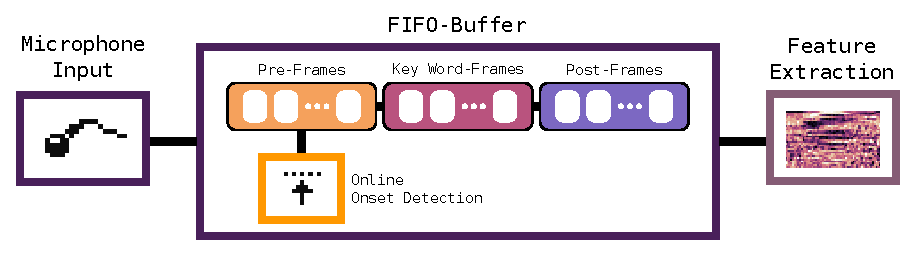
\includegraphics[width=0.60\textwidth]{./6_game/figs/game_system_fifo}
  \caption{FIFO buffer structure for the online system.}
  \label{fig:game_system_fifo}
\end{figure}
\FloatBarrier
\noindent
Note that the feature extraction has to use the same feature extraction parameters as the model was trained in the classification system.


% --
% classification

\subsection{Classification System}
The classification system consists of a classifier, which is composed of a neural network architecture for the classification of the key words (speech commands) it was trained for.
The trained weights of a neural network model are stored in the \texttt{.pth} format for the \texttt{Pytorch} framework.
A separate parameter file is stored to provide information of the unique model name (for example \texttt{conv-jim}) of the neural network architecture, the feature extraction parameters and the class dictionary.
Feature extraction parameters provide information of which constellation of features were used during training, for instance 12 MFCC coefficients frame-based normalized, so that the same extraction is applied for inference of new data samples from the online system.
The class dictionary describes which output node of the neural network corresponds to which speech command, this is especially important for the video game application to observe, which key word was spotted.
After the parameters are loaded, the classifier simply does an inference to the most probable key word in its class dictionary.

The game action can be performed once a key word is present from the classification system.
This for example can be implemented by using an input handler, similar to a keyboard input handler or event system, that is listening if a command is present and eliciting a corresponding action.

